\section{Σύστημα Γραμμικής Πρόβλεψης}

\par Το επόμενο βήμα για την υλοποίηση του συστήματος κωδικοποιητή αποκωδικοποιητή είναι η
δημιουργία ενός συστήματος Γραμμικής Πρόβλεψης. Συγκεκριμένα, καλούμαστε να σχεδιάσουμε ένα φίλτρο
\emph{m}-οστής τάξης το οποίο θα προβλέπει την επόμενη τιμή του σήματος με βάση τις m προηγούμενες.
Αναλυτικότερα:

\begin{equation}
  \label{eq:predictor}
  \hat{x}(n) = \sum_{i=1}^m w_i x(n -i)
\end{equation}
\noindent όπου $\hat{x}$ η εκτίμηση μας, $w_i$ το i-οστό βάρος και $x(n-i)$ μία από τις προηγούμενες
τιμές του σήματος. Η παραπάνω εξίσωση γράφεται με την μορφή διανυσμάτων ως:
\begin{equation}
  \label{eq:vectorized_predictor}
  \hat{x}(n) = \vec{w}^T\vec{x}
\end{equation}
\noindent όπου
\begin{equation}
  \label{eq:params_vector}
  \vec{w} = \begin{bmatrix}
    w_1 & \\
    w_2  \\
    \vdots \\
    w_m
  \end{bmatrix}
  \quad
  \vec{x} = \begin{bmatrix}
    x(n-1) & \\
    x(n-2)  \\
    \vdots \\
    x(n-m)
  \end{bmatrix}
\end{equation}
\par Το σφάλμα πρόβλεψης ορίζεται ως:
\begin{equation}
  \label{eq:pred_error}
  e = x(n) - \hat{x}
\end{equation}

\par Για να βρούμε τις παραμέτρους, επιλέγουμε να ελαχιστοποιήσουμε το μέσο τετραγωνικό σφάλμα:
\begin{equation}
  \label{eq:min_mse}
  \underset{\vec{w}}{argmin}{E\left[e^2(n)\right]}
\end{equation}
\noindent το οποίο και παραγωγίζουμε ως προς τα βάρη $w_i$ και θέτουμε ίσο με μηδέν, για να βρούμε
τα βάρη που αντιστοιχούν στο ελάχιστο:
\begin{align}
  &\frac{\partial J}{\partial \vec{w}} = 0 \label{eq:weight_calc1} \Rightarrow \\
  &\frac{\partial}{\partial \vec{w}}E[\left(x(n) - \vec{w}^T\vec{x}\right)\left(x(n) - \vec{w}^T\vec{x}\right)] = 0
  \label{eq:weight_calc2} \Rightarrow \\
  &E\left[\frac{\partial}{\partial \vec{w}}(\left(x(n) - \vec{w}^T\vec{x}\right)\left(x(n) -
      \vec{w}^T\vec{x}\right))\right] = 0 \label{eq:weight_calc3} \Rightarrow \\
  &-2E\left[(x(n) - \vec{w}^T\vec{x})\vec{x}^T\right]=0 \label{eq:weight_calc4}\Rightarrow \\
  &E[x(n)\vec{x}^T] = \vec{w}^TE[\vec{x}\vec{x}^T] \label{eq:weight_calc5} \Rightarrow \\
  &\vec{r}^T = \vec{w}^TR \label{eq:weight_calc6} \Rightarrow \\
  &R\vec{w}  = \vec{r} \label{eq:weight_calc7} \Rightarrow \\
  &\bm{\boxed{w = R^{-1}\vec{r}}}\label{eq:weight_calc8}
\end{align}
\noindent όπου ο πίνακας \emph{R} είναι ο πίνακας αυτοσυσχέτισης και το $\vec{r}$ το διάνυσμα
αυτοσυσχέτισης, τα οποία είναι ίσα με:
\begin{align}
  \label{eq:autocorr_mat}
  R = E&\begin{bmatrix}
    &x(n-1)x(n-1) & x(n-1)x(n-2) & \ldots & x(n-1)x(n-M) \\
    &x(n-2)x(n-1) & x(n-2)x(n-2) & \ldots & x(n-2)x(n-M) \\
    &\vdots &\vdots &\ddots & \ldots \\
    &x(n-M)x(n-1) & x(n-M)x(n-2) & \ldots & x(n-M)x(n-M) \\
  \end{bmatrix} \\
  R = &\begin{bmatrix}
    &r(0) & r(1) & \ldots & r(M - 1) \\
    &r(1) & r(0) & \ldots & r(M - 1) \\
    &\vdots &\vdots &\ddots & \ldots \\
    &r(M - 1) & r(M-2) & \ldots & r(0) \\
  \end{bmatrix}
\end{align}

\begin{equation}
  \label{eq:autocorr_vec}
  \vec{r} = E\begin{bmatrix}
    &x(n)x(n-1) \\
    &x(n)x(n-1) \\
    &\vdots \\
    &x(n)x(n-M)
  \end{bmatrix} = \begin{bmatrix}
    &r(1) \\
    &r(2) \\
    &\vdots \\
    &r(M)
  \end{bmatrix}
\end{equation}
\noindent όπου τα $r(i)$ είναι η τιμή της συνάρτηση αυτοσυσχέτισης για μετατόπισης του σήματος κατά \emph{i}
βήματα.

\par Η συνάρτηση που υλοποιεί την παραπάνω λειτουργικότητα είναι η:
\begin{lstlisting}[style=MyMatlab]
 function [w, varargout] = lpcoeffs(x, m, debug)
\end{lstlisting}
\par όπου \emph{x} είναι το σήμα μας, \emph{m} η τάξη του φίλτρου πρόβλεψης και τα \emph{debug},
\emph{varargout} είναι προαιρετικά ορίσματα εισόδου κι εξόδου που χρησιμοποιούνται για να ελέγξουμε την ορθότητα
του διανύσματος της αυτοσυσχέτισης που υπολογίζουμε. Για το σκοπό αυτά υλοποιήθηκε το script
\emph{autocorr\_tests} και η συνάρτηση \emph{test\_lpcoeffs\_autocorr} τα οποία συγκρίνουν τις παραπάνω
ποσότητες με τις αντίστοιχες που επιστρέφονται από τις built-in συναρτήσεις του MATLAB.


\noindent
\begin{minipage}{\linewidth}
  \par Στην συνέχεια, παραθέτουμε τα γραφήματα που προέκυψαν από την δοθείσα συνάρτηση ελέγχου για
  να δείξουμε την ορθή λειτουργία της συνάρτησης υπολογισμού των βαρών του φίλτρου.
  \begin{figure}[H]
    \label{fig:pred_filter1}
    \centering
    \begin{subfigure}{0.49\textwidth}
      \includegraphics[width=0.35\paperwidth]{lp1.eps}
      \caption{\protect{Πρόβλεψη AR διαδικασίας με φίλτρο τάξης 2}}
    \end{subfigure}
    \,
    \begin{subfigure}{0.49\textwidth}
      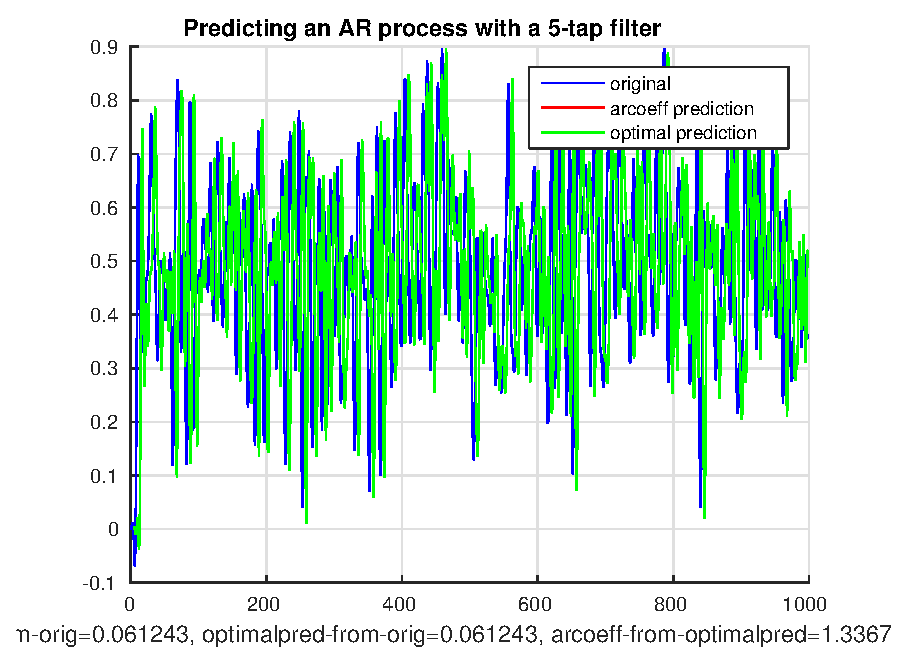
\includegraphics[width=0.35\paperwidth]{lp2.eps}
      \caption{\protect{Πρόβλεψη AR διαδικασίας με φίλτρο τάξης 5}}
    \end{subfigure}
    \\
    \begin{subfigure}{0.49\textwidth}
      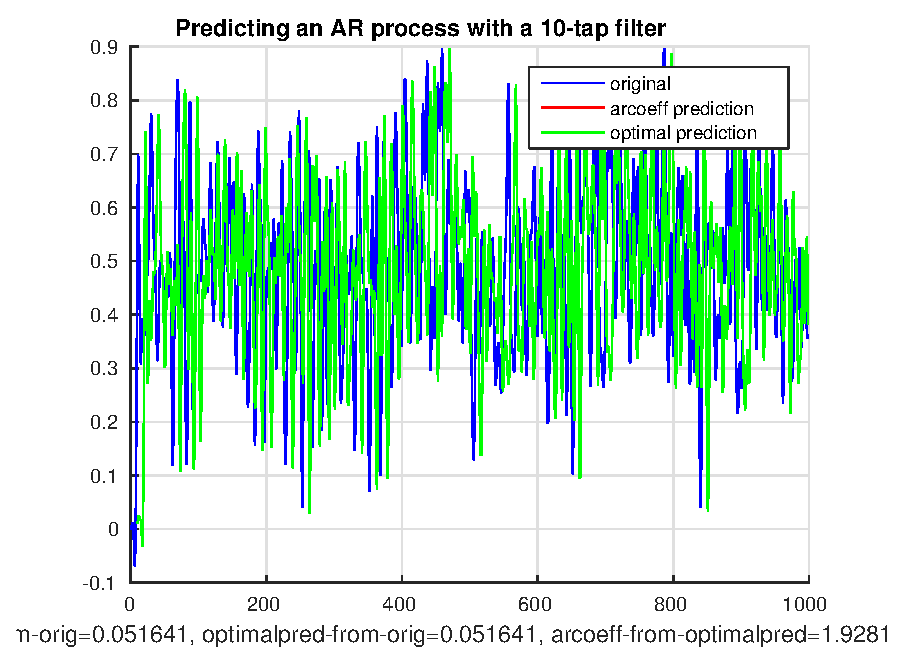
\includegraphics[width=0.35\paperwidth]{lp3.eps}
      \caption{\protect{Πρόβλεψη AR διαδικασίας με φίλτρο τάξης 10}}
    \end{subfigure}
    \caption{\protect{Αποτελέσματα Πρόβλεψης για διαδικασίες AR}}
  \end{figure}
\end{minipage}

\noindent
\begin{minipage}{\linewidth}
  \begin{figure}[H]
    \label{fig:pred_filter2}
    \centering
    \begin{subfigure}{0.49\textwidth}
      \includegraphics[width=0.35\paperwidth]{lp4.eps}
      \caption{\protect{Πρόβλεψη λευκού θορύβου με φίλτρο τάξης 2}}
    \end{subfigure}
    \,
    \begin{subfigure}{0.49\textwidth}
      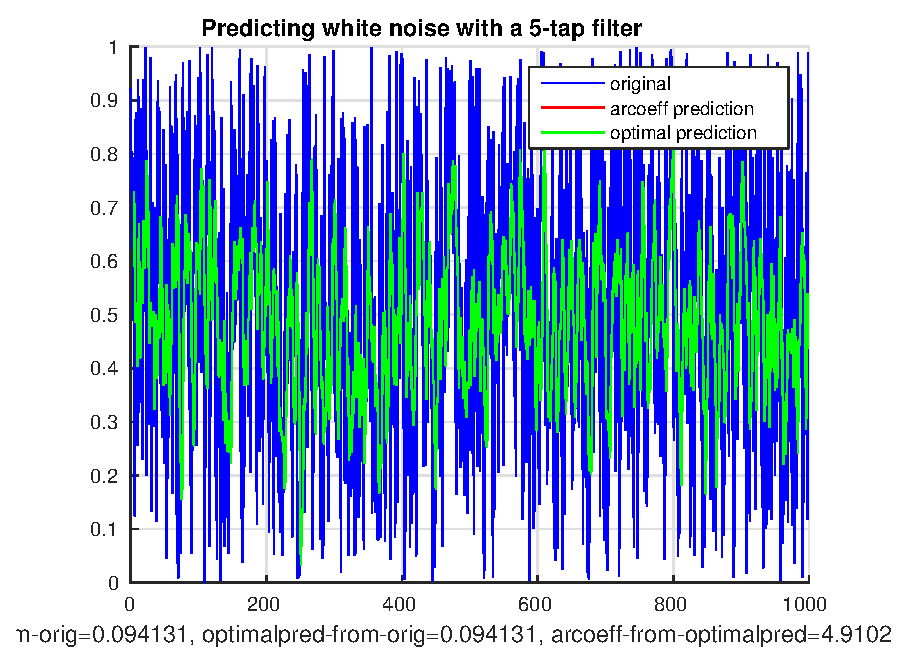
\includegraphics[width=0.35\paperwidth]{lp5.eps}
      \caption{\protect{Πρόβλεψη λευκού θορύβου με φίλτρο τάξης 5}}
    \end{subfigure}
    \begin{subfigure}{0.49\textwidth}
      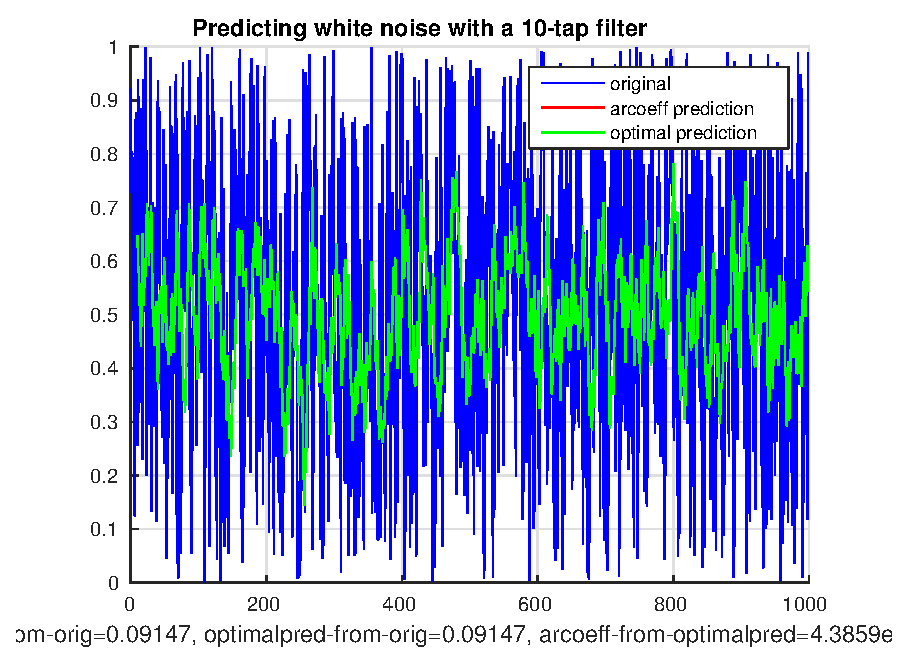
\includegraphics[width=0.35\paperwidth]{lp6.eps}
      \caption{\protect{Πρόβλεψη λευκού θορύβου με φίλτρο τάξης 10}}
    \end{subfigure}
    \caption{\protect{Αποτελέσματα Πρόβλεψης με είσοδο λευκό θόρυβο}}
  \end{figure}
\end{minipage}

\noindent
\begin{minipage}{\linewidth}
  \begin{figure}[H]
    \label{fig:pred_filter3}
    \centering
    \begin{subfigure}{0.49\textwidth}
      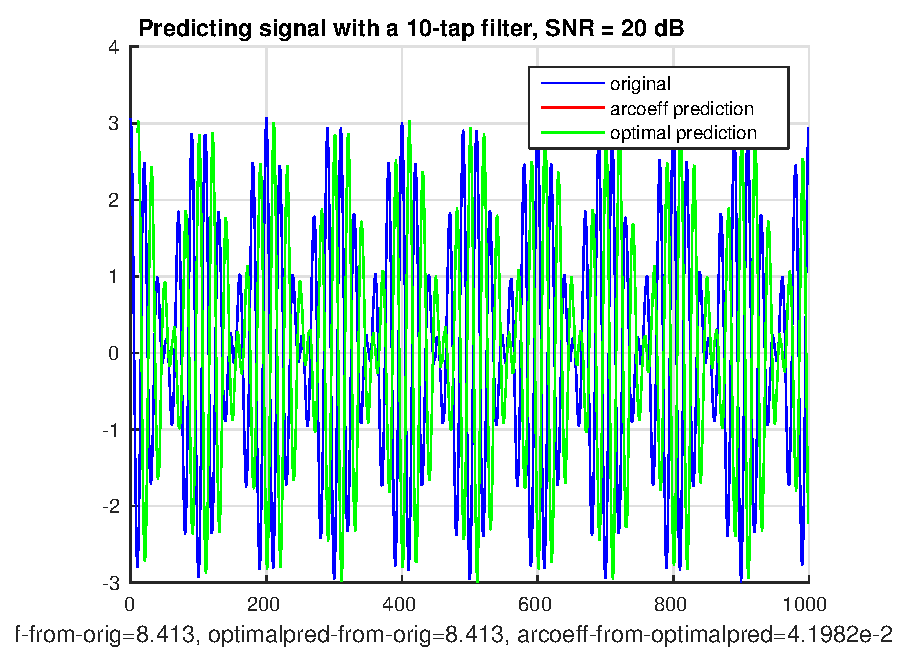
\includegraphics[width=0.35\paperwidth]{lp7.eps}
      \caption{\protect{Πρόβλεψη σήματος με φίλτρο τάξης 10 και SNR 20dB}}
    \end{subfigure}
    \,
    \begin{subfigure}{0.49\textwidth}
      \includegraphics[width=0.35\paperwidth]{lp8.eps}
      \caption{\protect{Πρόβλεψη λευκού θορύβου με φίλτρο τάξης 10 και SNR 17dB}}
    \end{subfigure}
    \\
    \begin{subfigure}{0.49\textwidth}
      \includegraphics[width=0.35\paperwidth]{lp9.eps}
      \caption{\protect{Πρόβλεψη λευκού θορύβου με φίλτρο τάξης 10 και SNR 13dB}}
    \end{subfigure}
    \,
    \begin{subfigure}{0.49\textwidth}
      \includegraphics[width=0.35\paperwidth]{lp10.eps}
      \caption{\protect{Πρόβλεψη σήματος με φίλτρο τάξης 10 και SNR 10dB}}
    \end{subfigure}
    \\
    \begin{subfigure}{0.49\textwidth}
      \includegraphics[width=0.35\paperwidth]{lp11.eps}
      \caption{\protect{Πρόβλεψη σήματος με φίλτρο τάξης 10 και SNR 5dB}}
    \end{subfigure}
    \caption{\protect{Πρόβλεψη σήματος μέσω γραμμικού φίλτρου πρόβλεψης}}
  \end{figure}
\end{minipage}

